\chapter{Release 3: Financial Management and Governance}

\section*{Introduction}
\addcontentsline{toc}{section}{Introduction}
This release delivers what the platform was commissioned for: replacing the financial logic of the
Excel workbook. Sprint~6 records the revenue side, that is billing milestones, payments and
amendments, together with the mission expenses that eat into the margin. Sprint~7 adds the
governance registers, which document the life of a project. Sprint~8 closes the loop with the
internal quote and the indicator engine. That engine reads everything built since Release~1.
\section{Sprint 6 --- Billing and missions}

\subsection{Sprint objectives}
Sprint~6 ran from 25~May to 12~June, three weeks (Table~\ref{tab:schedule}). Its objective is to
open the financial side. Milestones carry the invoicing, payments track what has been collected,
amendments move the budget, and missions bring travel cost into the project.

\subsection{Sprint backlog}
The sprint commits the following items of the product backlog (Table~\ref{tab:backlog}).

\begin{longtable}{|m{1.6cm}|m{12.4cm}|}
\caption{Sprint 6 backlog}\label{tab:sb6}\\
\hline
\textbf{Story} & \textbf{User story} \\
\hline
\endfirsthead
\hline
\textbf{Story} & \textbf{User story} \\
\hline
\endhead
\endfoot
\endlastfoot
\hline
US-20 & As a project manager, I want to define billing milestones following contractual progress \\
\hline
US-21 & As a project manager, I want to record payments received against a milestone \\
\hline
US-22 & As a project manager, I want to record amendments so the revised budget reflects contractual change \\
\hline
US-23 & As a project manager, I want to include travel costs in the project cost \\
\hline
\end{longtable}

\subsection{Task planning}
The author being the sole developer, each item was expanded directly into the technical work it
required rather than distributed across a team.

\begin{longtable}{|m{1.6cm}|m{12.4cm}|}
\caption{Sprint 6 task planning}\label{tab:tp6}\\
\hline
\textbf{Story} & \textbf{Technical work} \\
\hline
\endfirsthead
\hline
\textbf{Story} & \textbf{Technical work} \\
\hline
\endhead
\endfoot
\endlastfoot
\hline
US-20 & Milestone as a percentage of the effective budget, sum capped at 100\% in the service layer \\
\hline
US-21 & Payments kept as individual rows so partial settlements stay visible \\
\hline
US-22 & Amendment as the single writer of the revised budget \\
\hline
US-23 & Mission with typed components, each converted at the mission date before summation \\
\hline
\end{longtable}

\subsection{Design}
The sprint covers the use cases through which a project earns and spends outside labour: defining a
billing milestone, invoicing it, recording a payment against it, recording a contractual amendment,
and recording a mission with its expenses. All are reserved to the project manager, except the
amendment, which the director records because it changes the contract.

\begin{figure}[H]
  \centering
  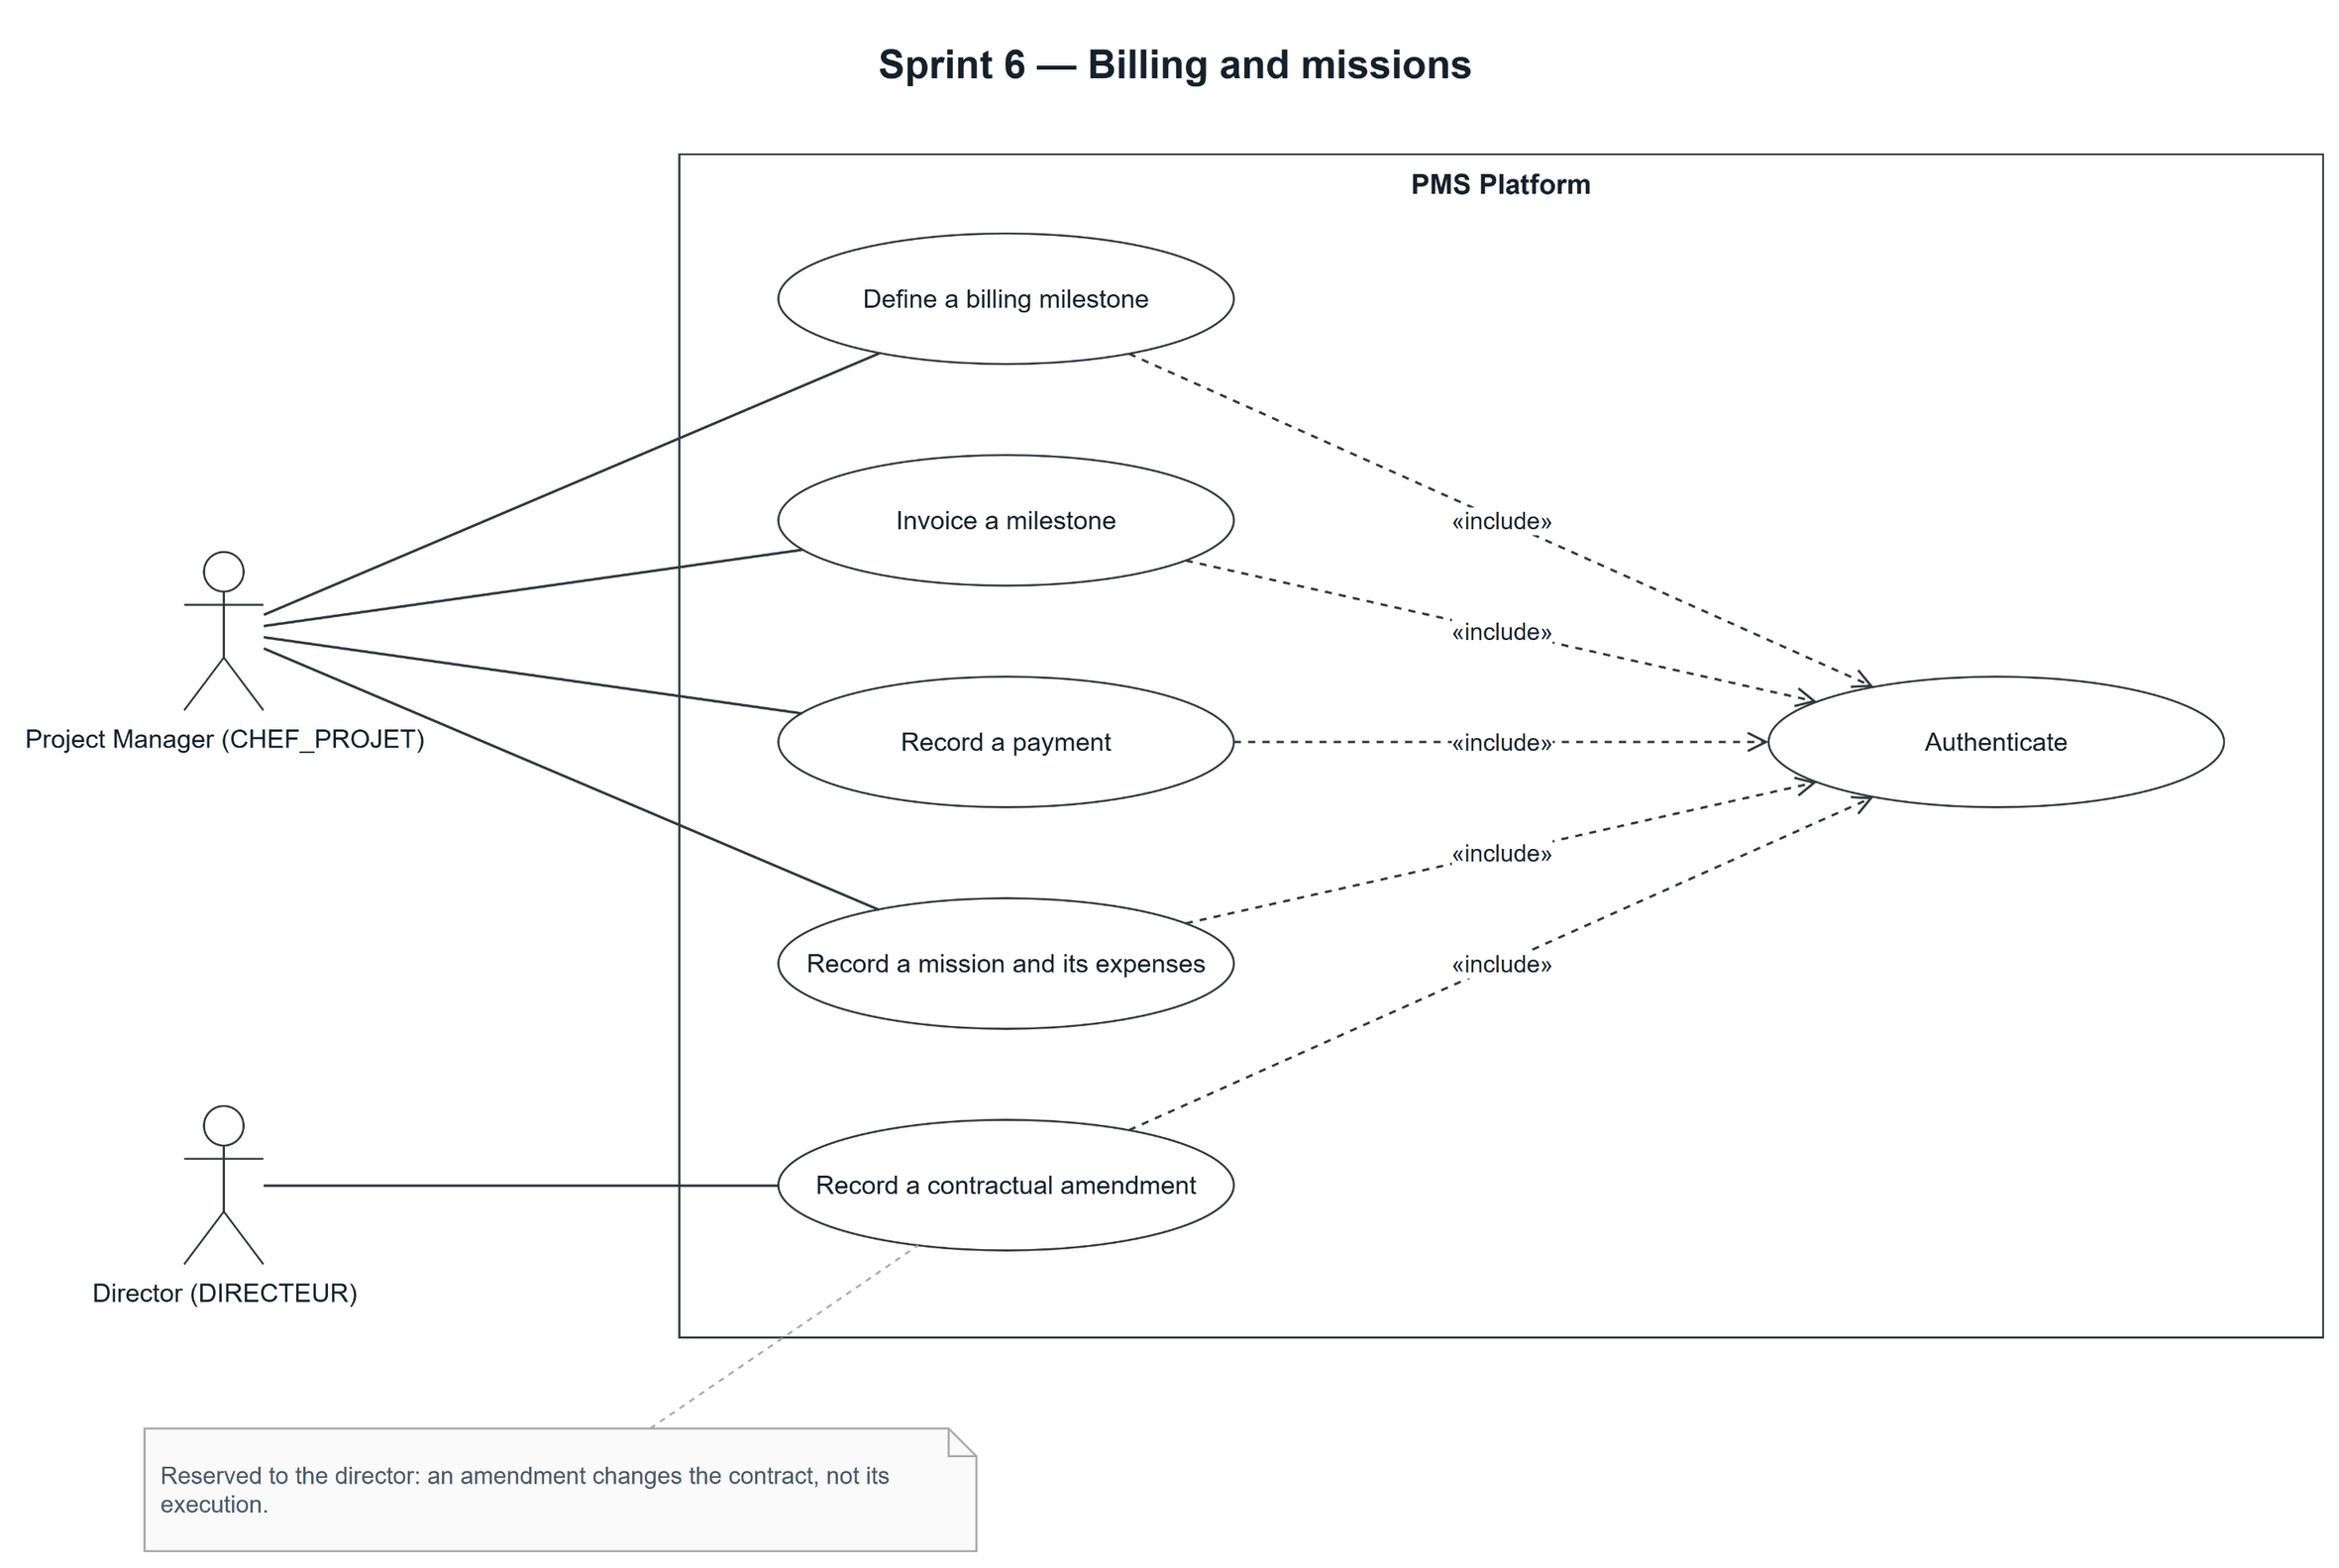
\includegraphics[width=0.75\columnwidth]{img/uc_sprint6.png}
  \caption{Use case diagram of sprint 6}
  \label{fig:uc-s6}
\end{figure}

\runin{Model of billing and missions}
A milestone belongs to one project and carries a label, a percentage of the contract, an amount, a
due date and a status. A mission belongs to a project and an employee, and decomposes into typed
cost components.

\begin{figure}[H]
  \centering
  
\includegraphics[width=0.95\columnwidth]{img/class_financial.png}
  \caption{Class diagram --- financial management}
  \label{fig:class-fin}
\end{figure}

\runin{Design decisions}
\textbf{The milestone amount is derived, not stored.} It follows from the effective budget and the
percentage, so an amendment propagates automatically to every milestone not yet invoiced. Storing
the amount would have required updating each milestone on every amendment, and any missed update
would have gone unnoticed.

\textbf{The sum of percentages may not exceed 100\%.} This rule is inherited from the workbook,
where it was a convention the spreadsheet could not enforce. Here it is checked in the service
layer, and an attempt to exceed it is rejected rather than silently accepted.

\textbf{Payments are rows, not a settled total.} Keeping a single settled amount would lose the
history of partial settlements, which is precisely what a project manager chasing collection needs
to see.

\textbf{Conversion happens before summation, never after.} A mission may be incurred in a currency
different from the reporting one. Each component is converted at the rate of the mission date and
only then summed. Summing first would add amounts expressed in different currencies, and the total
would be meaningless while still looking plausible.

\subsection{Implementation}
The module opens on the milestone, which carries the invoicing, and the amendment, which is the
only thing allowed to move the budget.


\runin{Milestone lifecycle}
A milestone moves through three states: planned, invoiced and paid. Invoicing records the invoice
date; a payment recorded against an invoiced milestone moves it to paid.

\runin{Amendments}
An amendment carries a reference, an amount and an impact on the sold workload. It is the single
writer of the revised budget introduced in Sprint~3, which is what keeps the contractual and
financial history coherent.

\begin{figure}[H]
  \centering
  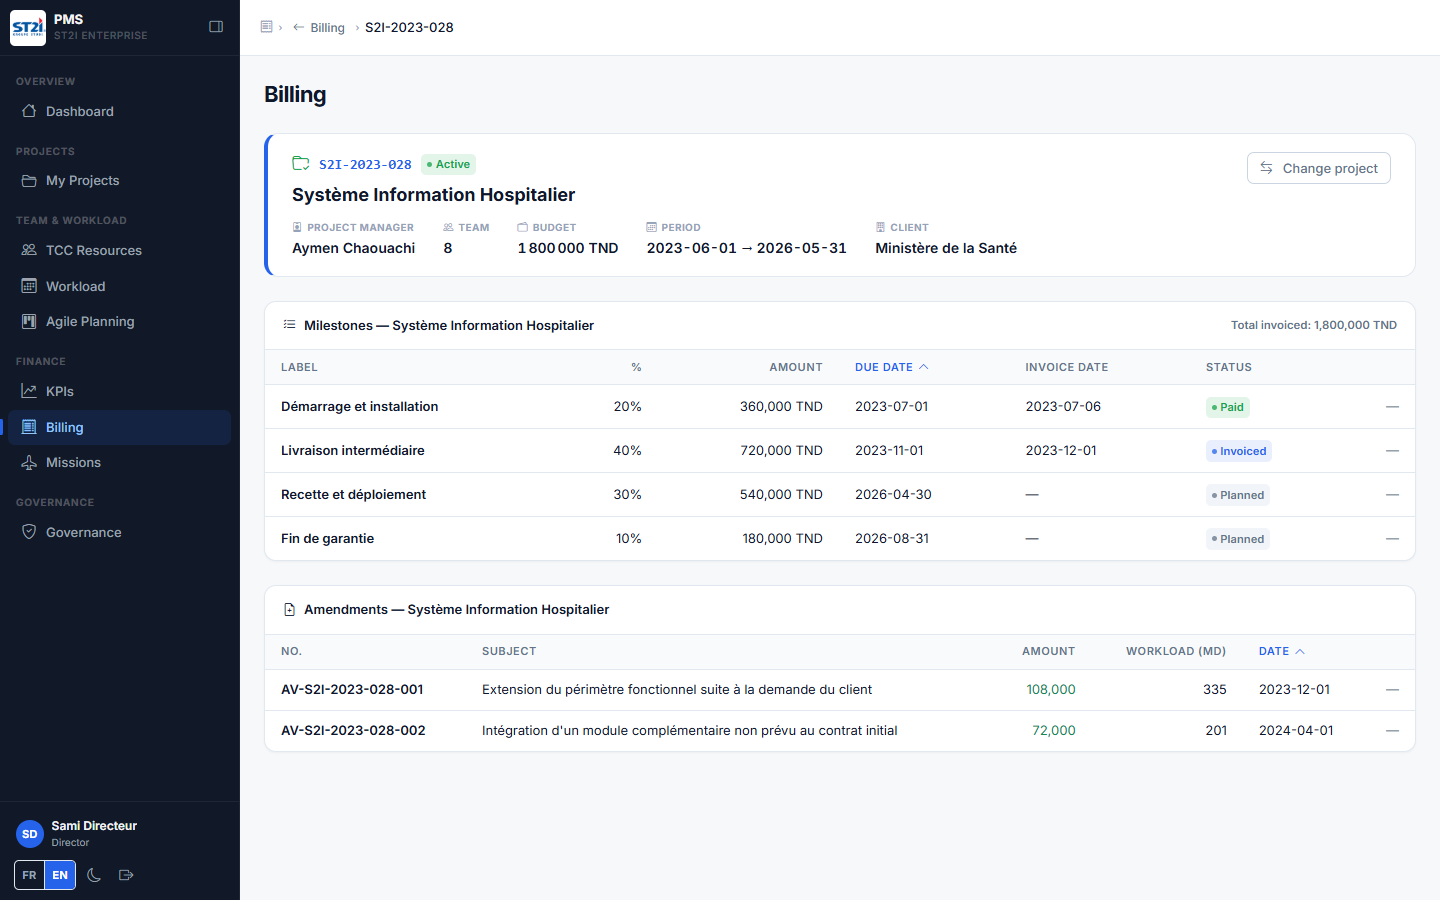
\includegraphics[width=0.95\columnwidth]{img/ui_billing.png}
  \caption{Billing milestones interface}
  \label{fig:ui-billing}
\end{figure}

Missions are recorded on their own screen, each one decomposed into the typed cost components
the workbook already used: per diem, ticket, transport, accommodation and stamp duty.

\begin{figure}[H]
  \centering
  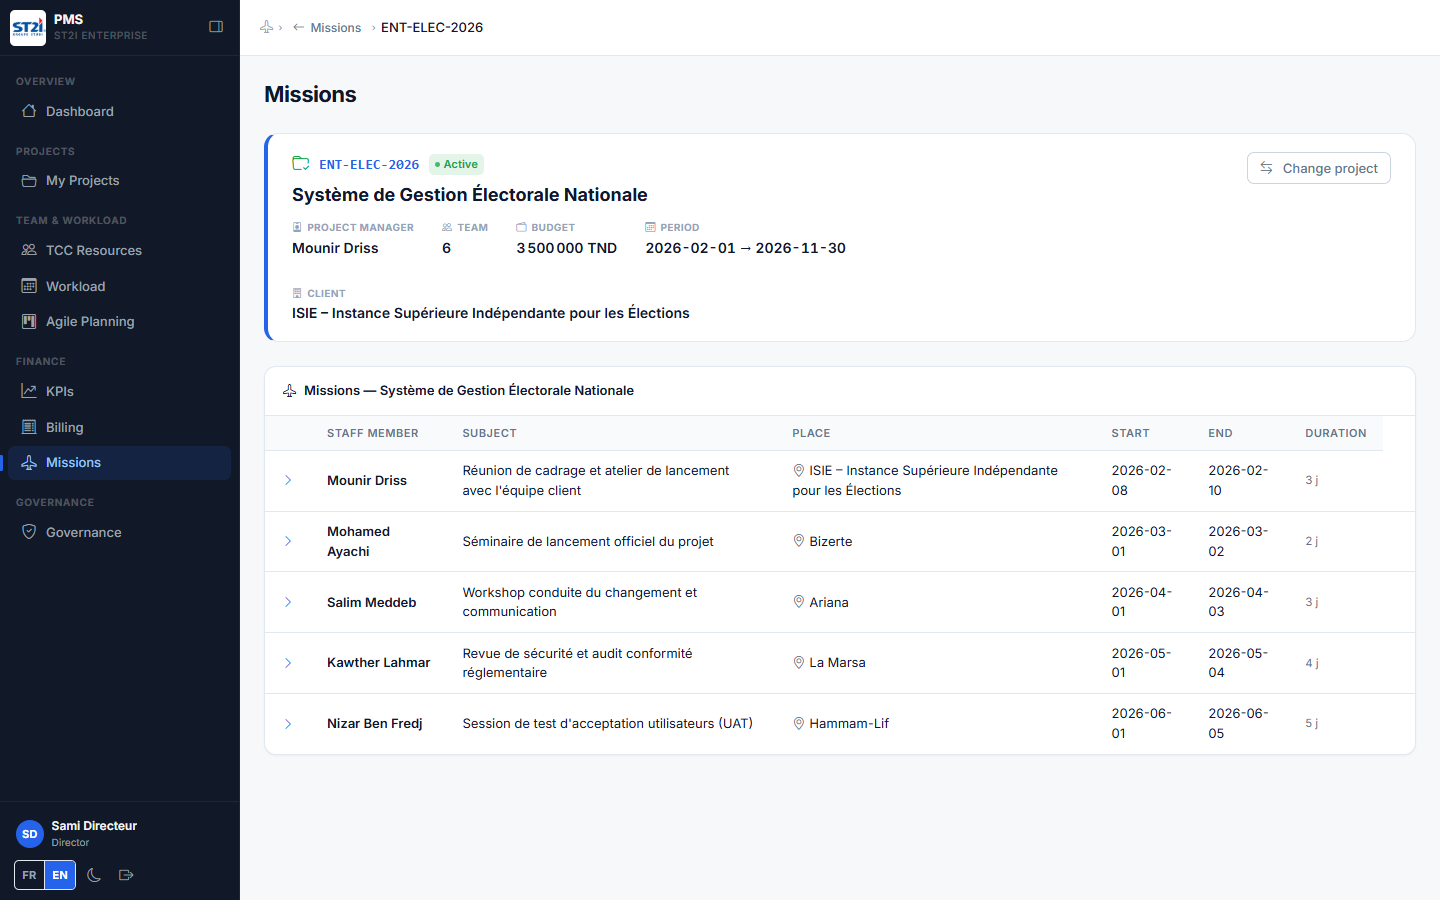
\includegraphics[width=0.95\columnwidth]{img/ui_missions.png}
  \caption{Missions interface, with the cost components of a mission expanded}
  \label{fig:ui-missions}
\end{figure}

\subsection{Testing}
The tests for this sprint sit with the module they check, and they run together with all the
others. They were run again for this report, and the counts below come from that run.

\textbf{\texttt{JalonServiceTest} (10 tests).} It checks the billing limit. A set of milestones
adding up to more than 100\% is refused, and one that adds up to exactly 100\% is accepted. It
then checks that a milestone already invoiced or paid cannot be invoiced again and cannot be
deleted. Last, it checks that the status is recomputed after a partial payment and after a full
one.

\textbf{\texttt{AvenantServiceTest} (5 tests).} It checks that the revised budget changes through
an amendment and in no other way.

\textbf{\texttt{BillingControllerTest} (8 tests).} It calls every endpoint of the module and
checks the permission each one requires.

That is 23 tests for this sprint, and all of them pass.

\subsection{Sprint review}
This review was the most literal of them all. The billing progress sheet of the workbook was
entered again, milestone by milestone, and the invoiced totals were compared line by line. The
limit on the sum of the percentages was checked first. The spreadsheet states that limit, but only
the platform enforces it.

% =====================================================================
\section{Sprint 7 --- Project governance}

\subsection{Sprint objectives}
Sprint~7 ran from 15~June to 3~July, three weeks (Table~\ref{tab:schedule}). Its objective is to
carry over the registers the workbook keeps beside the figures: risks, deliverables, stakeholders
and change requests. They are what makes a review a review rather than a balance sheet.

\subsection{Sprint backlog}
The sprint commits the following items of the product backlog (Table~\ref{tab:backlog}).

\begin{longtable}{|m{1.6cm}|m{12.4cm}|}
\caption{Sprint 7 backlog}\label{tab:sb7}\\
\hline
\textbf{Story} & \textbf{User story} \\
\hline
\endfirsthead
\hline
\textbf{Story} & \textbf{User story} \\
\hline
\endhead
\endfoot
\endlastfoot
\hline
US-24 & As a project manager, I want to keep a risk register \\
\hline
US-25 & As a project manager, I want to track deliverables and measure delivery progress \\
\hline
US-26 & As a project manager, I want to document the project stakeholders \\
\hline
US-27 & As a project manager, I want to record change requests \\
\hline
\end{longtable}

\subsection{Task planning}
The author being the sole developer, each item was expanded directly into the technical work it
required rather than distributed across a team.

\begin{longtable}{|m{1.6cm}|m{12.4cm}|}
\caption{Sprint 7 task planning}\label{tab:tp7}\\
\hline
\textbf{Story} & \textbf{Technical work} \\
\hline
\endfirsthead
\hline
\textbf{Story} & \textbf{Technical work} \\
\hline
\endhead
\endfoot
\endlastfoot
\hline
US-24 & Risk with probability, impact, status and mitigation plan \\
\hline
US-25 & Deliverable with a controlled status, feeding the delivery rate of the indicator engine \\
\hline
US-26 & Stakeholder register composed by the project, edited by the project manager \\
\hline
US-27 & Change request register composed by the project, each carrying a priority, a status and a decision date \\
\hline
\end{longtable}

\subsection{Design}
The sprint covers the four registers that document the qualitative life of a project: risks,
deliverables, stakeholders and change requests. The project manager maintains them; the director
consults them.

\begin{figure}[H]
  \centering
  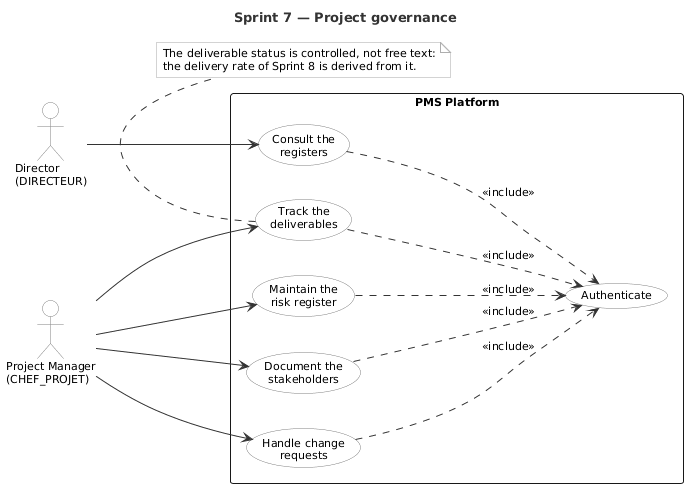
\includegraphics[width=0.75\columnwidth]{img/uc_sprint7.png}
  \caption{Use case diagram of sprint 7}
  \label{fig:uc-s7}
\end{figure}

\runin{Model of the governance registers}
The four registers share the same shape: each is composed by the project and governed by a small
business enumeration.

\begin{figure}[H]
  \centering
  
\includegraphics[width=0.95\columnwidth]{img/class_governance.png}
  \caption{Class diagram --- project governance}
  \label{fig:class-gov}
\end{figure}

\runin{Design decisions}
\textbf{The registers are attached to the project, not kept beside it.} Their value lies less in
their individual complexity than in belonging to the project itself, which the spreadsheet process
could not guarantee: risks and deliverables lived in separate documents that drifted from the
workbook.

\textbf{A deliverable carries a controlled status, not free text.} This is not documentation
tidiness. The delivery rate consumed by the indicator engine of Sprint~8 is derived from this
register, as the ratio of delivered and validated deliverables to planned ones. A free-text status
could not be counted, and the indicator would have had no input.

\textbf{Deletion is logical.} Removing an entry deactivates it and preserves the history, so that a
risk closed months ago remains visible in the record of how the project was steered.

\subsection{Implementation}
Each register exposes the same nested-resource shape under a project, with authorization carried by
the service layer and a dedicated pair of permissions separating consultation from modification.

\begin{figure}[H]
  \centering
  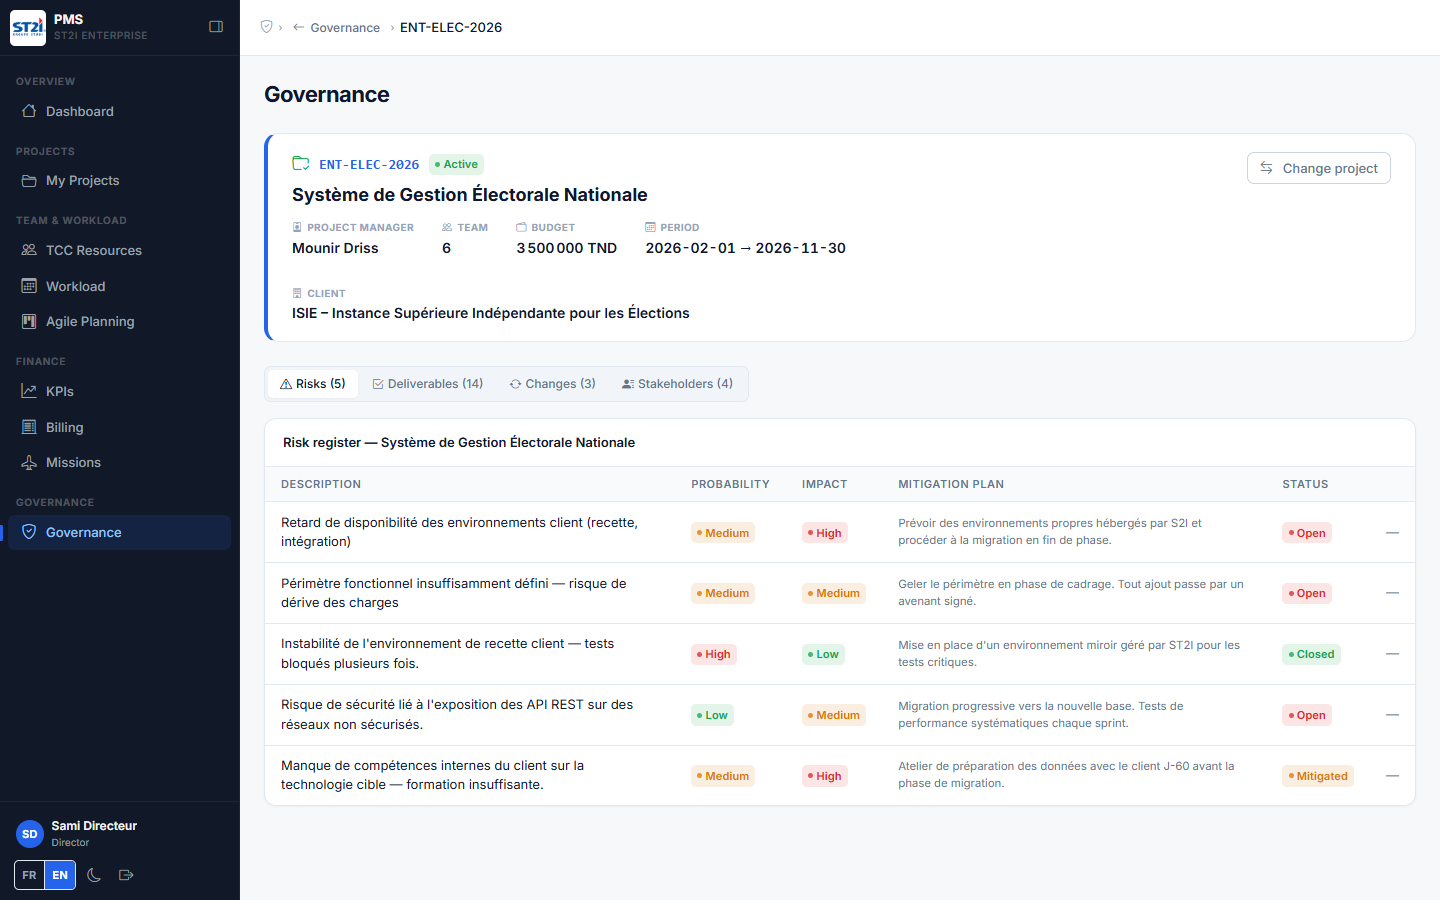
\includegraphics[width=0.95\columnwidth]{img/ui_governance.png}
  \caption{Governance interface}
  \label{fig:ui-gov}
\end{figure}

\subsection{Testing}
The tests for this sprint sit with the module they check, and they run together with all the
others. They were run again for this report, and the counts below come from that run.

\textbf{\texttt{GovernanceControllerTest} (8 tests).} It writes to each of the four registers and
reads them back, and checks the permission every endpoint requires.

All 8 of them pass.

\subsection{Sprint review}
The four registers were compared with the matching sheets of the workbook, field by field. One
point mattered more than the others. The status of a deliverable is chosen from a fixed list and
is not typed freely. The delivery rate of the next sprint reads that status, and free text would
have made the indicator impossible to compute.

% =====================================================================
\section{Sprint 8 --- Internal quote and indicator engine}

\subsection{Sprint objectives}
Sprint~8 ran from 6 to 24~July, three weeks (Table~\ref{tab:schedule}). Its objective is to close
the business scope with the part the whole project exists for: the economic baseline, and the
earned-value indicators the workbook computes by hand.

\subsection{Sprint backlog}
The sprint commits the following items of the product backlog (Table~\ref{tab:backlog}).

\begin{longtable}{|m{1.6cm}|m{12.4cm}|}
\caption{Sprint 8 backlog}\label{tab:sb8}\\
\hline
\textbf{Story} & \textbf{User story} \\
\hline
\endfirsthead
\hline
\textbf{Story} & \textbf{User story} \\
\hline
\endhead
\endfoot
\endlastfoot
\hline
US-28 & As a director, I want to give the project an economic baseline \\
\hline
US-29 & As a project manager, I want the financial indicators computed automatically \\
\hline
US-30 & As a project manager, I want to freeze a monthly review as history \\
\hline
US-31 & As a director, I want to supervise the whole portfolio \\
\hline
\end{longtable}

\subsection{Task planning}
The author being the sole developer, each item was expanded directly into the technical work it
required rather than distributed across a team.

\begin{longtable}{|m{1.6cm}|m{12.4cm}|}
\caption{Sprint 8 task planning}\label{tab:tp8}\\
\hline
\textbf{Story} & \textbf{Technical work} \\
\hline
\endfirsthead
\hline
\textbf{Story} & \textbf{Technical work} \\
\hline
\endhead
\endfoot
\endlastfoot
\hline
US-28 & Internal quote structured by section, gated by a dedicated permission \\
\hline
US-29 & Recompute-on-read engine valuing effort at the cost rate of its own year \\
\hline
US-30 & Immutable snapshot storing the indicators and the earned value entered by the manager \\
\hline
US-31 & Per-project and portfolio dashboards derived from the same engine \\
\hline
\end{longtable}

\subsection{Design}
The sprint covers the use cases that produce the figures the platform exists for: defining the
internal quote, consulting the computed indicators, freezing a monthly review, and consulting the
portfolio dashboard. The internal quote is reserved to the director alone.

\begin{figure}[H]
  \centering
  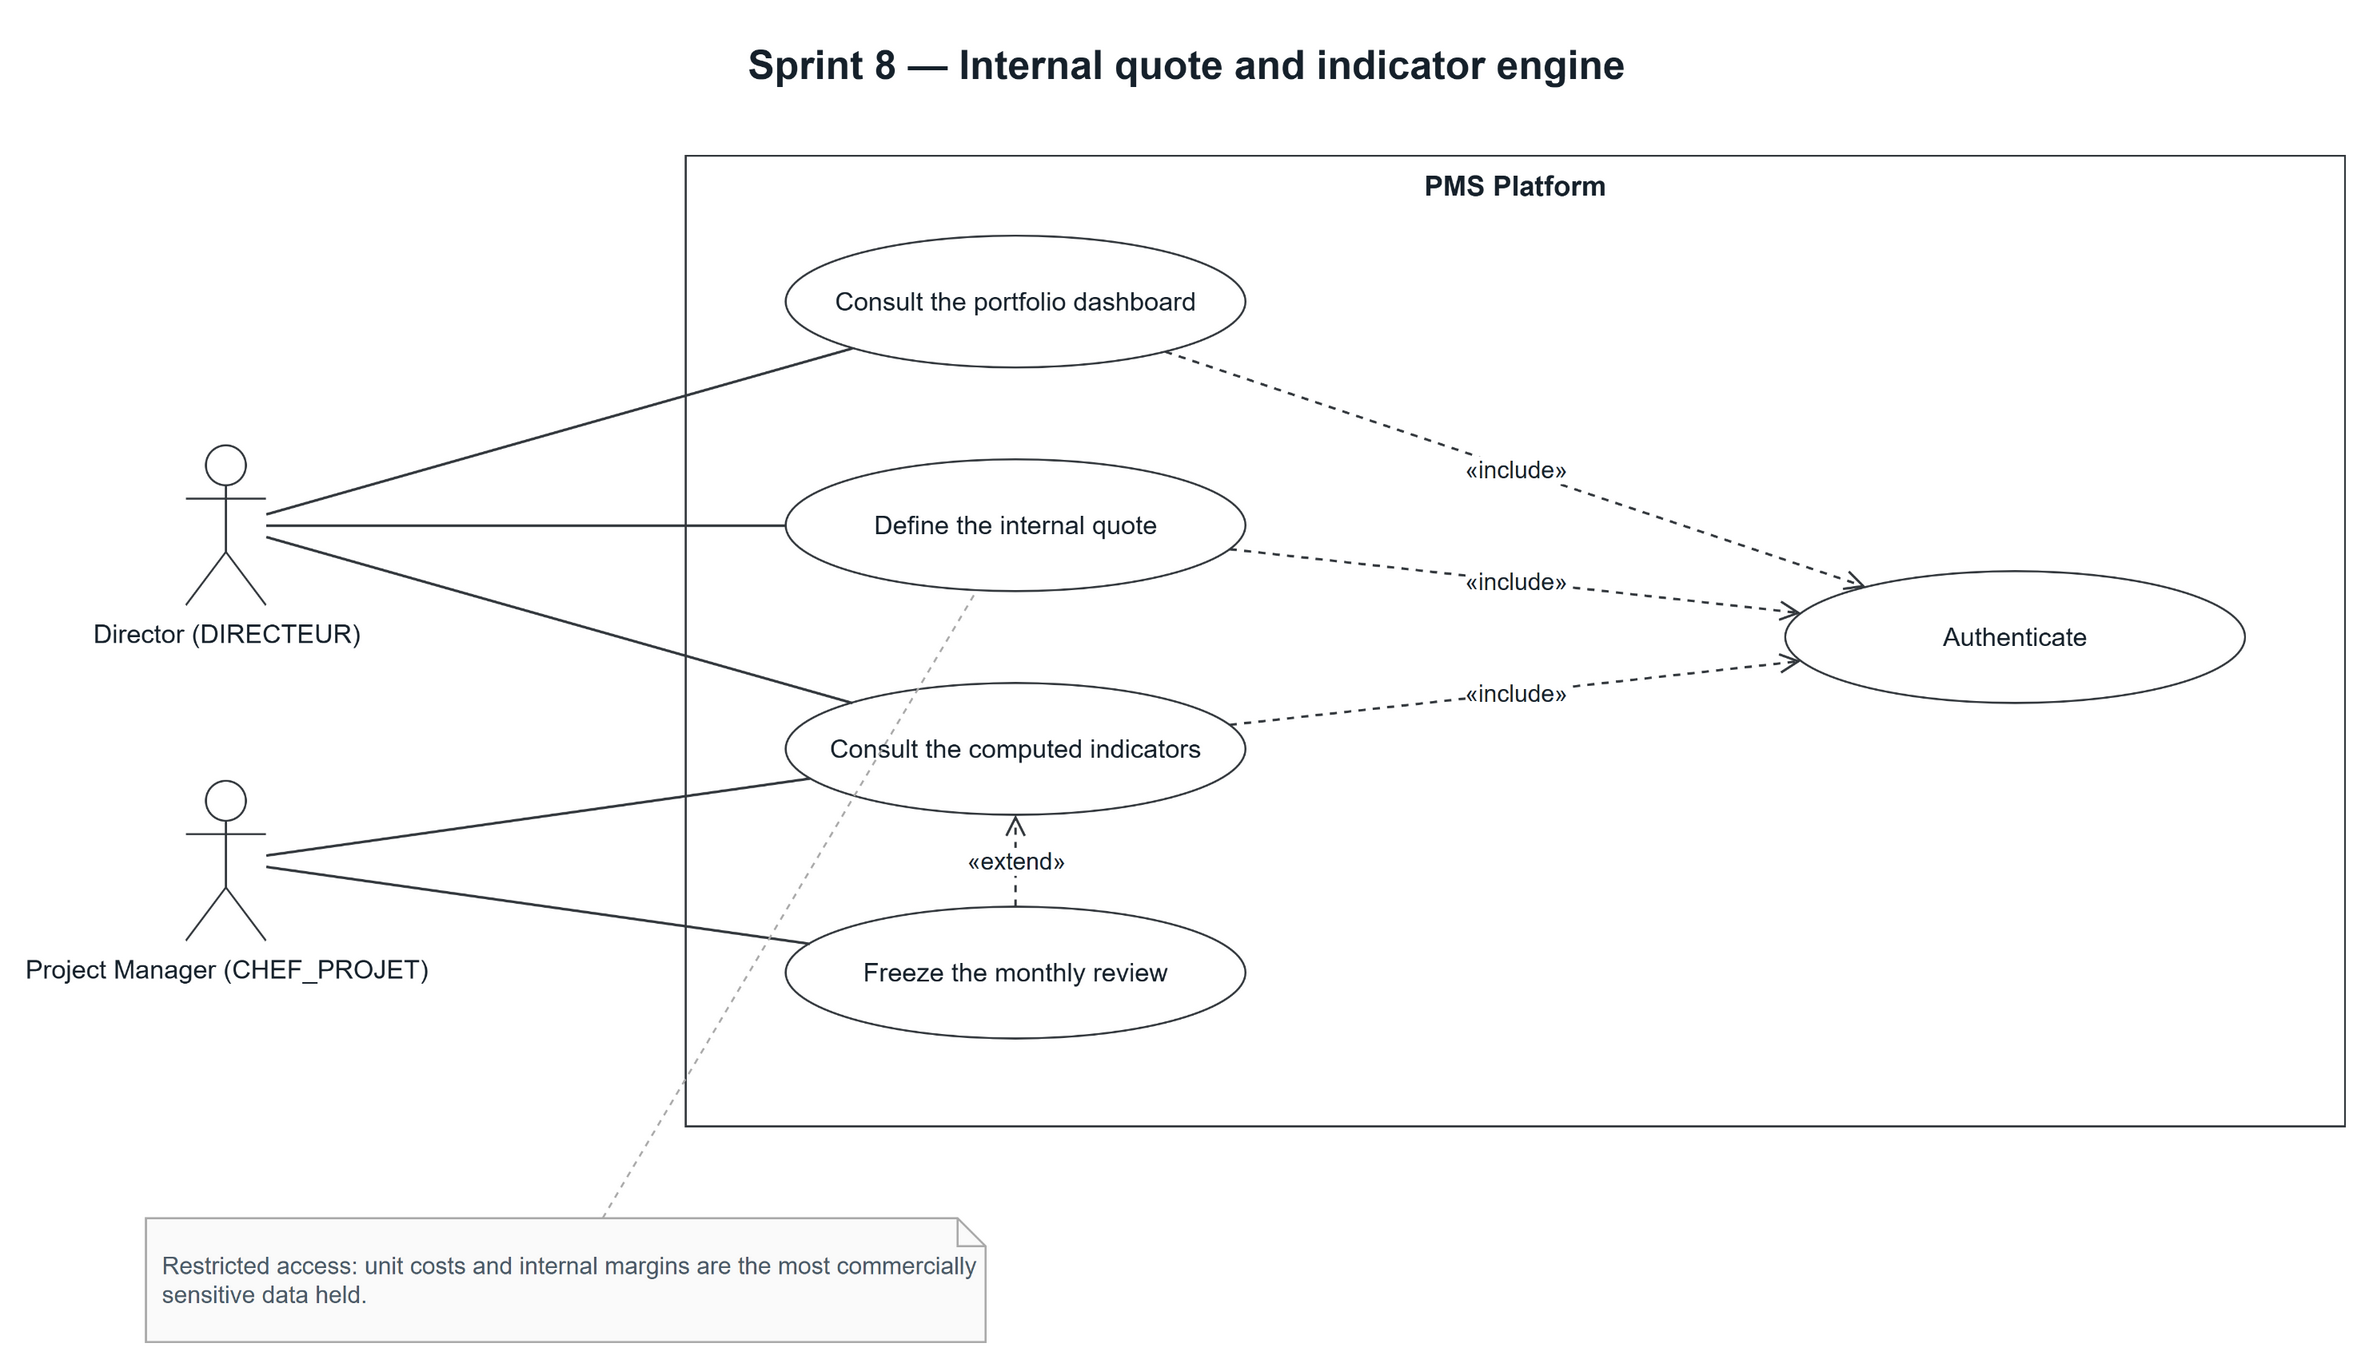
\includegraphics[width=0.75\columnwidth]{img/uc_sprint8.png}
  \caption{Use case diagram of sprint 8}
  \label{fig:uc-s8}
\end{figure}

\runin{Model of the indicator engine}
The engine reads from every module built since Release~1: workload for consumed and remaining
effort, cost rates for valuation, billing for invoiced revenue, and the deliverable register for
delivery progress.

\begin{figure}[H]
  \centering
  
\includegraphics[width=0.95\columnwidth]{img/class_kpi.png}
  \caption{Class diagram --- workload and indicator engine}
  \label{fig:class-kpi}
\end{figure}

\runin{Sequence from workload entry to frozen review}
Figure~\ref{fig:seq-kpi} shows the complete chain, from the submission of a month of effort to the
snapshot that freezes the monthly review.

\begin{figure}[H]
  \centering
  
\includegraphics[width=0.95\columnwidth]{img/seq_submit_workload.png}
  \caption{Sequence diagram --- workload entry and indicator computation}
  \label{fig:seq-kpi}
\end{figure}

\runin{Design decisions}
\textbf{Amounts and margins are never stored.} They are recomputed at read time from quantities,
unit values and the exchange rate. Persisting them would duplicate commercially sensitive figures
and allow the stored value to diverge from its inputs, which is exactly the failure the workbook
suffered when a formula was overwritten by a pasted constant.

\textbf{A read has no side effect.} Consulting a dashboard writes nothing. This is what makes the
indicators safe to display anywhere, and it is why two consecutive reads always agree.

\textbf{The earned value is entered, not computed.} The percentage of value earned is a judgement
made by the project manager during the monthly review, not a measurement the system can derive.
Pretending otherwise would have produced an indicator that looks objective and is not.

\textbf{The monthly review is frozen and immutable.} Submitting the review creates a snapshot of the
indicators of that month. This is the digital equivalent of the monthly column of the statistics
sheet: live figures for steering, frozen figures for history. A later correction cannot rewrite a
review a decision was already based on.

\textbf{The internal quote is gated by its own permission.} Unit costs and internal margins are the
most commercially sensitive data the platform holds, so access is not inherited from the project
role but granted explicitly and separately.

\subsection{Implementation}
The sprint delivers the baseline a project is measured against, and the engine that measures it.


\runin{The internal quote}
The quote is the economic baseline of the project: line items grouped by section, each carrying a
sold quantity and unit price on the revenue side, and an internal quantity and unit cost on the cost
side. The computation runs in two passes so that section subtotals and the overall margin remain
consistent with the line items they summarise.

\runin{The computed indicators}
On each read the engine recomputes, from live data, the indicators of the reference workbook:

\begin{itemize}
  \item \textbf{Actual cost} --- consumed man-days valued at the cost rate of their own year;
  \item \textbf{ETC} --- remaining man-days valued the same way;
  \item \textbf{EAC} --- actual cost plus ETC;
  \item \textbf{Production revenue} --- contract total weighted by the earned value percentage;
  \item \textbf{Accrued income} --- production revenue minus the invoiced total;
  \item \textbf{Margin} --- effective budget minus EAC, in value and in percentage;
  \item \textbf{Drift} --- sold workload minus consumed minus remaining.
\end{itemize}

Figure~\ref{fig:ui-kpi} shows them as the project manager reads them, each indicator
beside the value it is computed from.

\begin{figure}[H]
  \centering
  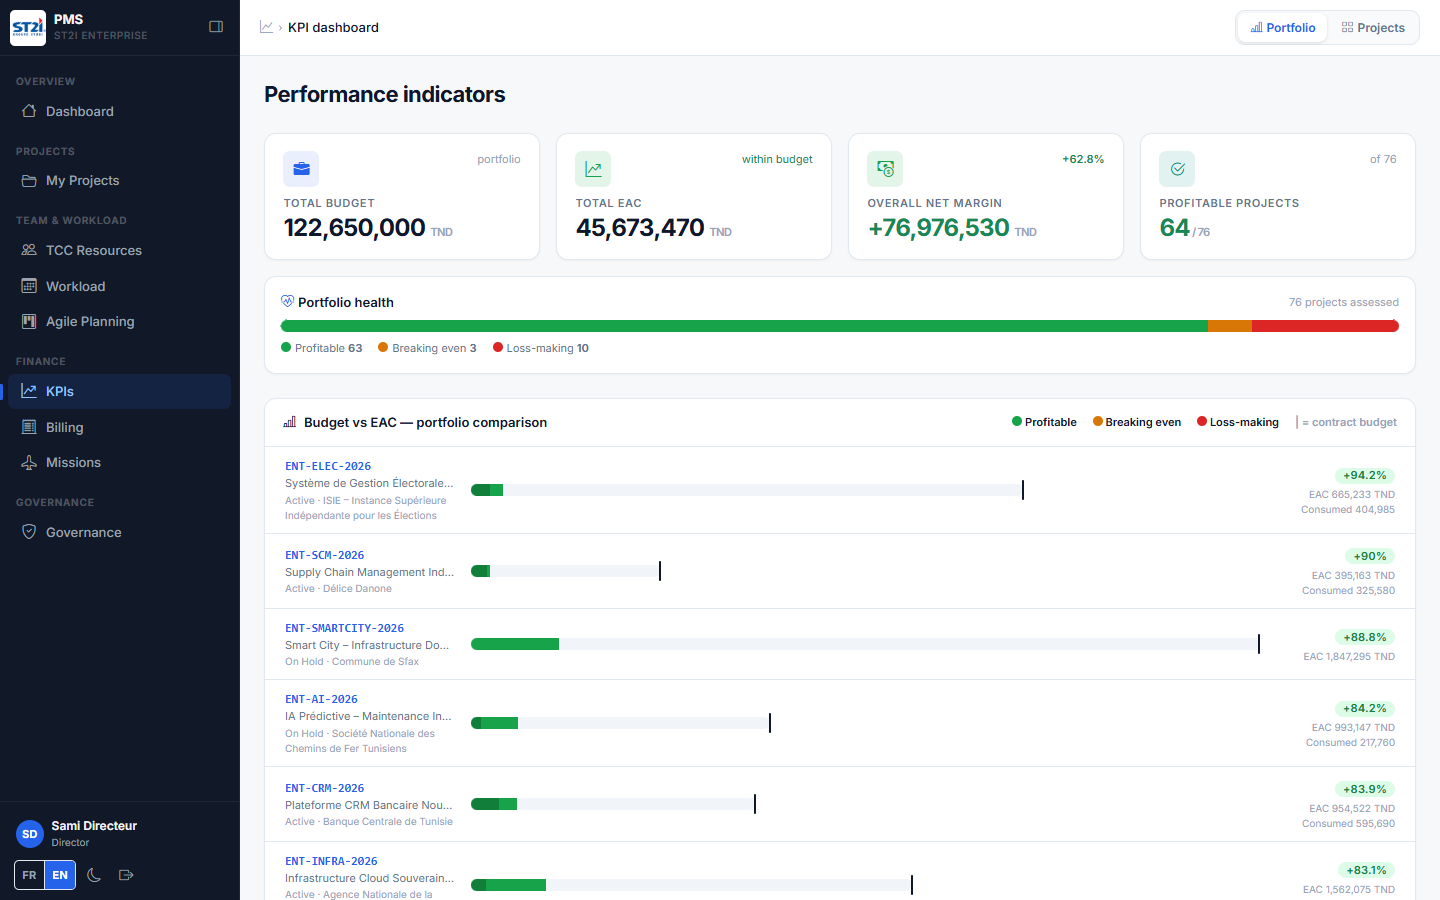
\includegraphics[width=0.95\columnwidth]{img/ui_kpi.png}
  \caption{KPI dashboard interface}
  \label{fig:ui-kpi}
\end{figure}

The same engine feeds the portfolio view of the director, which ranks every project by margin and
summarises the health of the whole portfolio in one bar. This is the screen that replaces the
manual consolidation the company had no way to automate: one workbook per project could be read
one at a time, never together.

\begin{figure}[H]
  \centering
  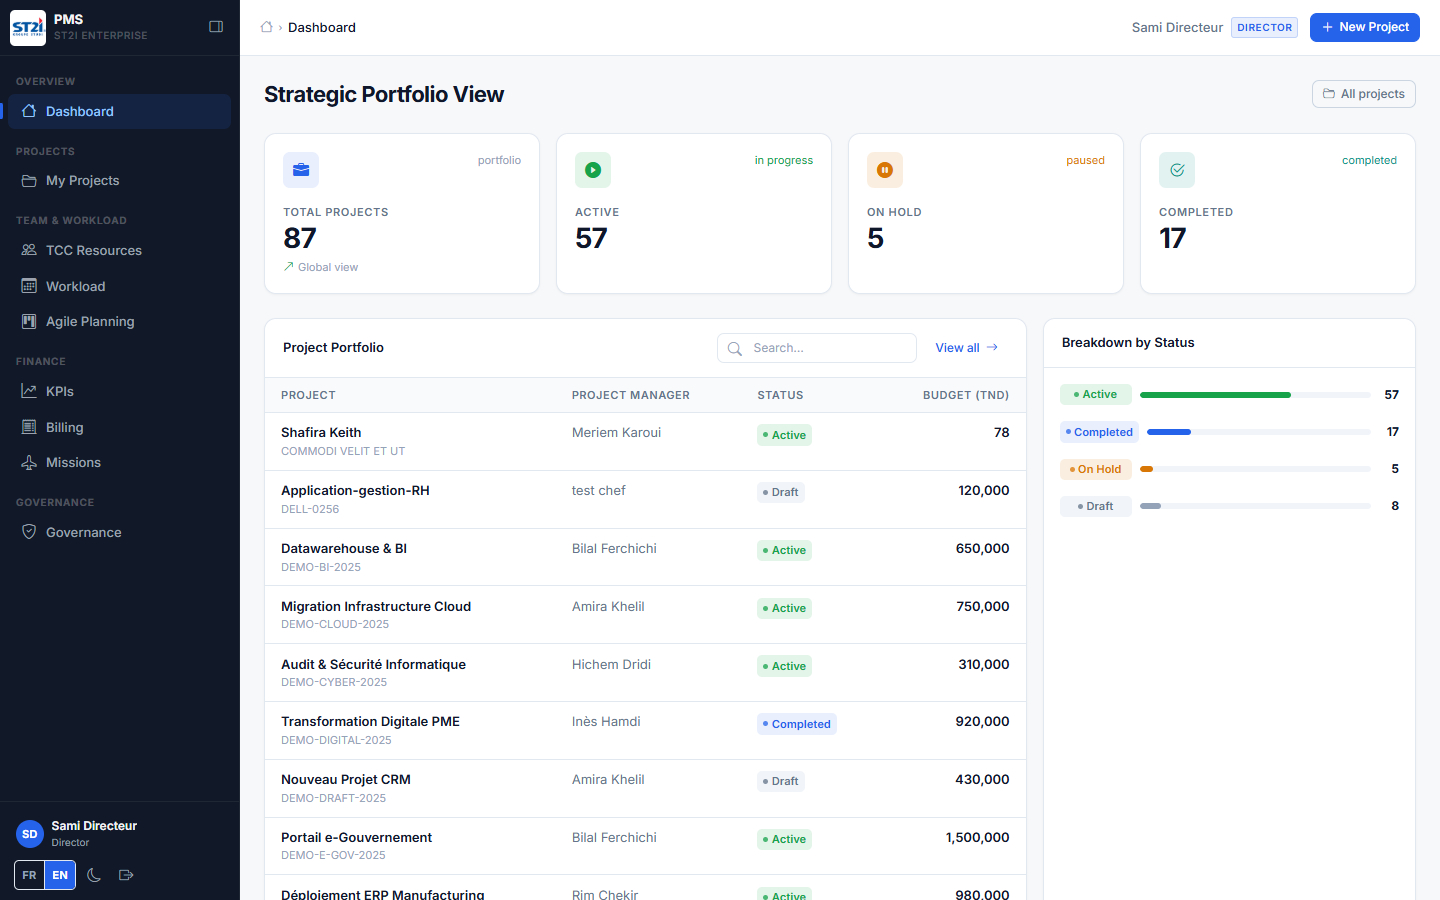
\includegraphics[width=0.95\columnwidth]{img/ui_dashboard.png}
  \caption{Portfolio dashboard of the director}
  \label{fig:ui-portfolio}
\end{figure}

\subsection{Testing}
The tests for this sprint sit with the module they check, and they run together with all the
others. They were run again for this report, and the counts below come from that run.

\textbf{\texttt{DevisInterneServiceTest} (4 tests).} It checks that the internal quote can be
reached only with its own permission.

\textbf{\texttt{KpiControllerTest} (6 tests).} It reads the indicators and the dashboards, and
checks that only the roles allowed to see financial data can reach them.

That is 10 tests for this sprint, and all of them pass.

\subsection{Sprint review}
The review was a direct comparison. One project was entered on the platform, then the indicators
were read twice: once in the workbook, once on the dashboard. Where the two figures differed, the
workbook was treated as correct and the engine was corrected. The workbook is the real
specification of the company.

% =====================================================================
\section*{Conclusion}
\addcontentsline{toc}{section}{Conclusion}
Release~3 delivered what PMS was commissioned for: billing and expenses, the governance registers,
the internal quote, and above all the indicator engine that replaces the two thousand formulas of
the reference workbook. The engine works in two ways. It computes live figures for steering, and
it freezes snapshots for history. This keeps what the spreadsheet did well and removes what made
it fragile.
